\chapter{Fundamentos te\'oricos}

\section{Antecedentes}

	Los estudios de datos longitudinales han cobrado cada vez m\'as importancia en el estudio de la epidemiolog\'ia, dando \'enfasis en los m\'odelos lineales mixtos, facilitando el desarrollo de m\'ultiples investigaciones y aplicaciones, buscando aprovechar el alcance para generar soluciones a problemas reales y modelos de dichas t\'ecnicas para diversas aplicaciones. Entre algunas de las investigaciones que sirvieron de base para este trabajo de grado son:\\

\textit{\citet{dengue}} realizaron un art\'iculo titulado: \textit{Modelado del efecto de la variabilidad clim\'atica local sobre la transmisi\'on de dengue en Medell\'in (Colombia) mediante an\'alisis de series temporales} para la revista Biom\'edica, Instituto Nacional de Salud, Colombia; en esta investigaci\'on se emple\'o la incidencia del dengue como variable dependiente y como variables independientes, los factores clim\'aticos registrados a escala semanal, utilizaron el programa expert modeler desarrollando un m\'odelo, explicando mejor el comportamiento de la enfermedad mediante el m\'odelo ARIMA, se seleccionaron las variables clim\'aticas que tuvieron una relaci\'on significativa con la variable dependiente. Se evidenci\'o una fuerte asociaci\'on entre el dengue y la precipitaci\'on permitiendo construir un m\'odelo que ayuda a comprender la din\'amica de transmisi\'on.  \\

\citet{latreia} realizaron un art\'iculo titulado: \textit{Ronda Cl\'inica y epidemiol\'ogica. An\'alisis de datos longitudinales} para la revista Latreia, Universidad de Antioquia, Medell\'in, Colombia; hacen un estudio de los datos longitudinales para evaluar de manera apropiada las medidas de un mismo sujeto que se repiten en el tiempo, indica que con esta herramienta es m\'as f\'acil entender los indicadores de cambio en procesos de salud y enfermedades, para la evaluaci\'on del efecto de diversas intervenciones ter\'apeuticas, se estudian los m\'odelos lineales mixtos.\\

\textit{\citet{tuberculosis}} realizaron un art\'iculo titulado: \textit{Tuberculosis en Barcelona: M\'odelo predictivo basado en series temporales} para la Revista Espa\~nola de Salud P\'ublica, Ministerio de Sanidad, servicios sociales e igualdad, Madrid, Espa\~na; resaltan los m\'odelos predictivos basados en series temporales que fueron utilizados en Catalu\~na con la gripe, us\'andolos como base en el estudio de la tuberculosis, se han asignado a partir de 1987 hasta 2008 la fecha de inicio del tratamiento, agreg\'andose la incidencia cada 4 semanas, formando dos series temporales, una para aut\'octonos y otra para inmigrantes con una longitud cada una de 287 observaciones. El an\'alisis estad\'istico lo realizaron con el paquete estad\'istico R, lo que arrojo como resultados que en la poblaci\'on aut\'octona no present\'o una media constante a los largo de los a\~nos y en la poblaci\'on inmigrante present\'o una tendencia creciente a lo largo de todo el estudio. La conclusi\'on a la que llegan en el estudio es que las tendencias de nuevos casos de tuberculosis presentaron patrones diferentes en la poblaci\'on de aut\'octonos y la de inmigrantes. El procedimiento usado es sencillo de implementar y muy \'util para predecir futuros valores de series temporales con diferentes tendencias.\\

\citet{hiv} realiz\'o un trabajo especial de grado titulado: \textit{Comparative causal effect estimation and robust variance for longitudinal data structures with applications to observational HIV treatment} para la Universidad de California, Berkeley, Estados Unidos; esta investigaci\'on discute la aplicaci\'on y el desempe\~no comparativo de los estimadores robustos dobles para estimar el resultado medio espec\'ifico de la intervenci\'on en ajustes longitudinales sin confundir la funci\'on del tiempo as\'i como las variaciones correspondientes del estimador. En concreto, se centra en definir cuidadosamente los par\'ametros causales para evitar problemas de positividad conocidos, estimando estos par\'ametros utilizando la estimaci\'on basada en la p\'erdida m\'inima, compar\'andola con otros estimadores dobles robustos del mismo par\'ametro causal y estimando las variaciones correspondientes de una forma que demuestre errores v\'alidos de Tipo I, manteniendo al mismo tiempo la potencia estad\'istica.  Se utiliz\'o la estimaci\'on m\'inima basada en p\'erdidas para estimar el resultado medio espec\'ifico de la intervenci\'on utilizando estimadores de candidatos adaptativos de aprendizaje de m\'aquina de datos para los par\'ametros de molestia. Se abordan cuestiones pr\'acticas, que incluyen definir cuidadosamente los par\'ametros causales y permanecer dentro de los l\'imites implicados por el modelo estad\'istico mientras se utilizan los algoritmos de aprendizaje autom\'atico.\\

\citet{mixed} realiz\'o un trabajo especial de grado titulado: \textit{Handling incomplete high-dimesional multivariate longitudinal data with mixed data types by multiple imputation using a longitudinal factor analysis model} para la Universidad de California, Los Angeles, Estados unidos; desarroll\'o un modelo de imputaci\'on que resuelve el problema de datos faltantes basado en un an\'alisis de factores y un modelo de efectos mixtos lineales. La cadena de Markov Monte Carlo se utiliza para ajustar el modelo, dibujar par\'ametros, variables latentes y valores p\'erdidos iterativamente. El modelo de imputaci\'on fue escrito en un paquete R, probando el modelo de imputaci\'on desarrollado utilizando conjuntos de datos simulados en 32 escenarios y 2 hipot\'eticos, falta de datos de los mecanismos. Dos modelos competitivos PAN (Imputaci\'on M\'ultiple para Panel Multivariado o Datos en Cl\'uster) y MICE (Imputaci\'on M\'ultiple usando Ecuaciones Encadenadas) tambi\'en probados de la misma manera para comparaci\'on, para mostrar la necesidad de abordar el tipo de datos de alta dimensi\'on y mixto continuo. En comparaci\'on con la ejecuci\'on de la simulaci\'on, la evaluaci\'on del programa R en una sola computadora, el programa utilizado para la evaluaci\'on de la simulaci\'on se ejecut\'o aproximadamente 600 veces m\'as r\'apido. En el escenario m\'as desfavorable probado, el coeficiente cuadr\'atico subyacente es tan grande como 0,8 del coeficiente lineal, las tasas reales de cobertura de las estimaciones de intervalos del 95\% empiezan a descender por debajo del 90\%. Una aplicaci\'on a los datos de una odontolog\'ia se muestran, en comparaci/'on con el PAN, NORM y un corredor anterior del m\'etodo recientemente desarrollado.\\

\citet{health} realiz\'o un trabajo especial de grado titulado: \textit{Implementation, evaluation and application of multiple imputation for missing data in longitudinal electronic healt record research} para la Universidad de Londres, Reino Unido; los registros de salud electr\'onicos longitudinales son un recurso valioso para la investigaci\'on porque contienen informaci\'on sobre muchos pacientes durante largos per\'iodos de seguimiento. Lo cual se propuso adaptar, evaluar e implementar el doble algoritmo para imputar datos faltantes de grandes base de datos de atenci\'on. Para lograr esto, primero investigaron la extensi\'on y los patrones de los datos faltantes en un estudio cl\'inico longitudinal para los indicadores de salud asociados con el riesgo de enfermedad cardiov\'ascular para determinar si es plausible. Adem\'as, desarroll\'o m\'etodos para identificar y eliminar los valores at\'ipicos, es decir, de datos con mediciones repetidas antes de la imputaci\'on. Finalmente, aplic\'o el doble algoritmo en THIN para modelar el riesgo de enfermedad cardiov\'ascular y entender los factores asociados con una mayor reducci\'on del colesterol total en pacientes con diabetes tipo II. \\

\citet{life} realiz\'o un paquete de R titulado: \textit{HIV calibrated model life tables for countries with generalized HIV epidemics} para el repositorio de R \textit{CRAN}; las funciones en este paquete producen un conjunto completo de tasas de mortalidad como una funci\'on de una combinaci\'on de la prevalencia del VIH y la esperanza de vida al nacer, la mortalidad infantil, o mortalidad infantil con mortalidad adulta.\\

\citet{jm} realiz\'o un paquete de R titulado: \textit{Join modeling of longitudinal and survival data} para el repositorio de R \textit{CRAN}; un ensayo cl\'inico aleatorizado en el que se recopilaron datos longitudinales y de supervivencia para comparar
la eficacia y seguridad de dos medicamentos antirretrovirales en el tratamiento de pacientes que fracasaron o que fueron intolerante a la terapia con zidovudina (AZT).

\section{Bases te\'oricas}

	Este apartado presenta una fundamentaci\'on te\'orica de los principales conceptos y teor\'ias usadas en esta investigaci\'on, como lo son los datos longitudinales, an\'alisis de los datos longitudinales, an\'alisis temporal y VIH; los cuales sirven como soporte, necesarios para lograr el desarrollo de los objetivos propuestos. 
	
	\subsection{Estudios longitudinales}
	
	Son estudios de cohortes o seguimiento, implica mediciones repetidas, estas mediciones son tomadas en intervalos de tiempo entre la exposici\'on y el comienzo de la enfermedad, requiere de la experiencia de la poblaci\'on a largo plazo. Este estudio se basa en que un mismo individuo es observado en m\'as de una ocasi\'on, lo cual lo diferencia de los estudios de seguimiento, en los que los individuos son seguidos hasta la ocurrencia de un suceso tal, como la muerte o una enfermedad \citet{delgado}\\
	
	Los estudios longitudinales se dividen en dos grandes componentes, est\'an reflejados los datos longitudinales y los datos panel, haciendo referencia a los datos panel, han estado \'ultimamente en muchos trabajos de investigaci\'on, esto en gran parte, al avance en las bases de datos, lo cual hace la recolecci\'on de estos datos de individuos a lo largo del tiempo. Las condiciones son sencillas, debe haber individuos al cual, se les va a realizar la observaci\'on durante un determinado tiempo, lo cual representa una dimensi\'on temporal, pero estos datos son usados frecuentemente en estudios econom\'etricos.\\
	
	En esta  investigaci\'on solo estar\'a centrada en los datos longitudinales, puesto que implica m\'as de dos mediciones a lo largo de un seguimiento, es necesario m\'as de dos, lo cual es una ventaja a la hora de realizar el estudio de los datos de los individuos. Aunque hay una mayor probabilidad que existan datos un poco inconclusos, pacientes que hayan decidido abandonar el tratamiento, y estos datos son faltantes.

	
	\subsection{An\'alisis de datos longitudinales}
	
	Los an\'alisis de estos datos, incorporan un enfoque diferente, aprovech\'andose de las mediciones repetidas en los sujetos a lo largo del tiempo, permitiendo una inferencia, no solo poblacional sino a nivel individual en los cambios de un proceso a lo largo del tiempo o en las transiciones entre diferentes estados de salud y la enfermedad; tambi\'en puede evaluar y separar los efectos de cohorte y edad, pueden formular la dependencia en el tiempo de este efecto, y un seguimiento sobre los acumulados hasta el inicio del mismo, asociando la exposici\'on y efecto en cualquier momento de la historia de los pacientes y la exposici\'on act\'ua. \citet{delgado} 

\subsection{Datos longitudinales en el VIH}

	En particular, los datos longitudinales han demostrado el efecto de la infecci\'on del VIH como indicador de una funci\'on inmunol\'ogica como el conteo de las c\'elulas $T^{+}CD4$. Todo ello, con unas caracter\'isticas base como la carga viral, inmediatamente despu\'es del diagn\'ostico de la seroconversi\'on, asociado con un declive del conteo de las c\'elulas $T^{+}CD4$. \textit{\citet{belle}}
	
	El cuadro 2.1 refleja que entre m\'as alta sea la carga viral, mayor ser\'a la reducci\'on de las c\'elulas $T^{+}CD4$.
	
\begin{table}[H]
\begin{center}
\begin{tabular}{|l|l|l|l|}
\hline
\multicolumn{4}{|c|}{L\'inea base de carga viral} \\ \hline
A\~no & Bajo & Medio & Alto \\ \hline
0-1 & 744.8 & 638.9 & 600.3 \\ \hline
1-2 & 721.2 & 588.1 & 511.8 \\ \hline
2-3 & 645.5 & 512.8 & 474.6 \\ \hline
3-4 & 604.8 & 470.0 & 353.9 \\ \hline

\end{tabular}
\caption{Media de CD4 y el error est\'andar en el tiempo. Se dan res\'umenes separados para los grupos definidos por el nivel basal de la carga viral. Belle, G. (2004).}
\label{tabla:cd4}
\end{center}
\end{table}	

	En cada panel del recuento de $T^{+}CD4$ para un solo sujeto se representa frente a los tiempos que obtuvieron mediciones. Tales mediciones permiten la inspecci\'on de los patrones de respuesta individuales y si existe una fuerte heterogeneidad en las trayectorias. Adem\'as, los individuos pueden ser evaluados para el cambio en el tiempo. En la Figura 2.1 indica la mayor\'ia de los sujetos son m\'as o menos estables en sus mediciones con el tiempo, o tienden a ser decreciente.
	
	\begin{figure}[H]
	\centering
	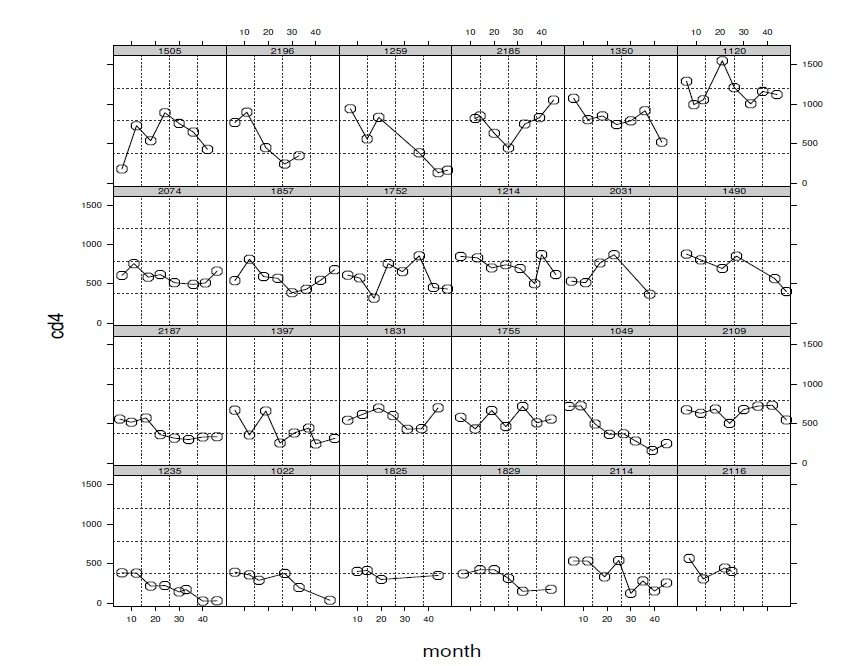
\includegraphics[scale=0.5]{datos.jpg}
	\caption{Una muestra de trayectorias CD4 individuales de los datos del Estudio Multi-Centro de Cohorte contra el SIDA. Belle, G. (2004).}
	\end{figure}
	
	En la situaci\'on com\'un en el que se est\'a interesado en la correlaci\'on de los resultados medidos a factores tales como el grupo de tratamiento o exposici\'on tambi\'en ser\'a \'util para graficar series individuales por el grupo de covarianza. \textit{\citet{belle}}

\subsection{M\'odelos lineales mixtos}

	Muchos m\'odelos estad\'isticos se pueden expresar como m\'odelos que incorporan dos partes: una parte son los efectos fijos, son par\'ametros asociados a toda la poblaci\'on o ciertos niveles de factores experimentales repetibles; otra parte son los efectos al azar, est\'an asociados con los sujetos experimentales o unidades extra\'idas u observados al azar de la poblaci\'on. Los m\'odelos con ambos, tanto el efecto fijo y el efecto al azar se denominan m\'odelos mixtos. \\
	 
	Los m\'odelos mixtos se utilizan principalmente para describir las relaciones entre una dimensi\'on-variable de respuesta final o multidimensional y algunas covariables posiblemente relacionados con los datos observados, agrupandose de acuerdo con uno o m\'as factores de agrupamiento. Tales datos deben incluir datos longitudinales, datos de medidas repetidas.\citet{zhang} 
	 
	 Para un solo nivel de agrupaci\'on de datos correlacionados, los m\'odelos lineales mixtos especifican la $n_{i}-dimensional$ responde al vector $Y_{i}=(Y_{i1},Y_{i2},\cdots ,Y_{inj})^{T}$ para $i=1,2,\cdots,m,$ con un n\'umero total de observaciones $\sum_{i=1}^m n_{i}$ 
	
	\begin{equation}
	 Y_{i}=X_{i}\beta +Z_{i}b_{i}+\epsilon_{i},   i=1,2,\cdots,m,	
	\end{equation}
	
	 \begin{equation}
	 b_{i} \sim N(0,\Psi),    \epsilon_{i} \sim N(0,\delta^{2}\Lambda_{i}),
	 \end{equation}

\noindent
Donde $\beta$ es el vector p-dimensional de efectos fijos \\
los $b_{i}$ son los vectores q-dimensionales de efectos al azar \\
$X_{i}$ son $n_{i} \times p$ matrices regresivas de efectos fijos \\
$Z_{i}$ son $n_{i} \times q$ matrices regresivas de efectos al azar \\
$\epsilon_{i}$ son las $n_{i}-$dimensionales sin un grupo de vectores de errores \\
$\psi$ es una matriz definida sim\'etrica positiva denotando la estructura de la varianza y covarianza entre los efectos al azar \\
$b_{i}$, $\lambda_{i}$ son matrices definidas positivas denotando la estructura de la varianza y la covarianza dependientes sin grupo de errores.\\ 

Los efectos al azar $b_{i}$ y el grupo sin errores $\epsilon_{i}$ se asumen que son independientes para los diferentes grupos y para ser independientes entre s\'i con el mismo grupo. En los modelos lineales mixtos, se supone que la respuesta continua gaussiana es una funci\'on lineal de covariables con coeficientes de regresi\'on que var\'ian sobre los individuos, lo que refleja la heterogeneidad natural debido a factores no medidos. \citet{zhang} 

\subsection{M\'odelos lineales mixtos en el an\'alisis de datos longitudinales}

	En medicina, se utilizan estudios longitudinales para descubrir factores predictivos de enfermedades. Los datos recogidos en un estudio longitudinal son datos longitudinales. En el an\'alisis de datos longitudinales, los modelos lineales mixtos son ampliamente utilizados. Medidas repetidas en datos longitudinales se observan en los sujetos a lo largo del tiempo. Adem\'as de la variable de tiempo, normalmente se observan otras covariables, lo que a su vez requiere una selecci\'on m\'as precisa para buscar el mejor modelo de una gran cantidad de modelos de candidatos. En el an\'alisis de los datos longitudinales por modelos lineales mixtos, la selecci\'on del modelo tambi\'en implica la selecci\'on de covariables y la variaci\'on de la selecci\'on de la estructura de covarianza de los efectos aleatorios y los errores dentro del grupo.\\
	
	En la figura 2.2. Toma una muestra y traza l\'ineas para cada sujeto estratificado por el nivel de carga viral de referencia. Esta cifra sugiere que la mayor carga viral del grupo tiene el menor recuento de $T^{+}CD4$, y sugiere que la variaci\'on entre las mediciones tambi\'en pueden ser menores para el grupo de carga viral basal, en comparación con los grupos medio y bajo. La figura 2.2 tambi\'en se puede usar para identificar las personas que exhiben tendencias temporales que difieren notablemente de otras personas. En el grupo de alta carga viral hay un individuo que parece mejorar dram\'aticamente con el tiempo, y hay una sola medici\'on inusual, donde el recuento de $T^{+}CD4$ es superior a 2000. El trazado de series individuales es un preludio exploratorio a un an\'alisis estad\'istico confirmatorio m\'as cuidadoso.
	
	\begin{figure}[H]
	\centering
	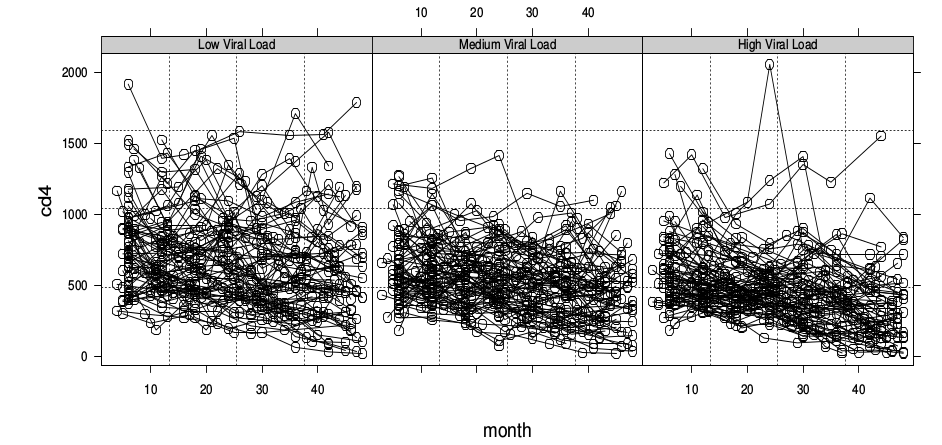
\includegraphics[scale=0.4]{mixed.png}
	\caption{Las trayectorias $T^{+}CD4$ individuales de los datos de la carga viral. Belle, G. (2004).}
	\end{figure}
	
\subsection{VIH}

	El virus de la inmunodeficiencia humana es un retrovirus o virus de \'acido ribonucleico (ARN), la conversi\'on de ARN en \'acido desoxirribonucleico (ADN) es la caracter\'istica definitoria del virus, la cual se lleva a cabo mediante la acci\'on enzim\'atica de la transcriptasa inversa. \\

	Seg\'un la \citet{oms}, el VIH puede trasmitirse por las relaciones sexuales vaginales, anales u orales con una persona infectada, la trasfusi\'on de sangre. Asimismo, puede trasmitirse de la madre al hijo durante el embarazo, el parto y la lactancia.\\

	La infecci\'on por VIH es silenciosa, porque no muestra ning\'un s\'intoma y suele ser diagnosticado por medio del estudio llamado: ensayo inmunoenzimatico ligado a enzimas (ELISA). \citet{bcs}
	
\subsection{SIDA}
	
	Se denomina as\'i, al cuadro cl\'inico que presenta los estadios m\'as avanzados de la infecci\'on por VIH, es decir; se considera cuando la cuenta de linfocitos $T^{+}CD4$ se encuentra por debajo de las 200 c\'elulas en un mililitro o cuando presenta el cuadro complejo de combinaci\'on de coinfecciones relacionadas con el VIH. \citet{bcs}	

\subsection{Relaci\'on VIH - $\mathrm{T^{+}CD4 - T^{+}CD8}$}

	Dos pruebas se pueden utilizar para monitorear el avance del VIH, son los recuentos de las c\'elulas $T^{+}CD4$ y las pruebas de carga viral. Los recuentos de $T^{+}CD4$ indican el estado del sistema inmunitario. Las pruebas de carga viral indican que tan activo est\'a el VIH. Al comienzo estas pruebas deben hacerse con 2 a 4 semanas de diferencia para establecer el “punto de partida” (baseline). Luego deben repetirse aproximadamente cada 3 meses. Las pruebas de carga viral, los recuentos de $T^{+}CD4$, proveer\'a una imagen m\'as clara sobre el riesgo que la enfermedad avance, el estado del sistema inmunitario y la capacidad del organismo para combatir el VIH.\\

	Normalmente, las pruebas sobre el recuento de los varios tipos de gl\'obulos blancos. Un tipo de gl\'obulos blancos son las c\'elulas B, las cuales est\'an involucradas en la producci\'on de anticuerpos. Las c\'elulas B tambi\'en se enfrentan a las infecciones que est\'an por fuera de las c\'elulas. Otro tipo de gl\'obulos blancos son las c\'elulas $T^{+}CD8$, las cuales se enfrentan a las infecciones por dentro de las c\'elulas. El tercer tipo de gl\'obulos blancos son las c\'elulas $T^{+}CD4$, las cuales ayudan a las c\'elulas B y $T^{+}CD8$ a llevar a cabo su labor. Estos gl\'obulos blancos se denominan linfocitos. \\ 

	En las personas VIH negativas, los recuentos normales de $T^{+}CD4$ fluct\'uan entre 600 y 1,500/$mm^{3}$. El recuento normal de $T^{+}CD8$ es de 300 a 800/$mm^{3}$. En general, una persona VIH negativa tiene 2 c\'elulas $T^{+}CD4$ por cada c\'elula $T^{+}CD8$ en la sangre. Sin embargo, en la enfermedad del VIH, el virus normalmente ocasiona una lenta disminuci\'on progresiva de las c\'elulas $T^{+}CD4$, y entre los que no est\'an en terapia para el VIH es com\'un ver invertida la relaci\'on entre $T^{+}CD4$ y $T^{+}CD8$. \\

	Los recuentos normales de $T^{+}CD4$ en las personas con VIH son de 350 a 800. Adem\'as de observar estos recuentos de c\'elulas, es tambi\'en \'util observar los porcentajes relativos de c\'elulas $T^{+}CD4$ y $T^{+}CD8$. El porcentaje de $T^{+}CD4$ es el porcentaje de c\'elulas $T^{+}CD4$ del total del recuento de gl\'obulos blancos. El rango normal es del 28 al 58\%. Un porcentaje de $T^{+}CD4$ por debajo del 14\% indica un diagn\'ostico de SIDA. \citet{ramduth} 
	
\subsection{Clasificaci\'on establecida de la infecci\'on por el VIH y enfermedades relacionadas}

	Seg\'un la Organizaci\'on Mundial de la Salud, en 1990 se desarroll\'o un sistema de estadificaci\'on cl\'inica de 4 estadios a efectos cl\'inicos que solo est\'a basado en adultos. Las clasificaciones cl\'inicas de los centros para el control y la prevenci\'on de enfermedades de los Estados Unidos y de la OMS, reconocen la infecci\'on primaria por el VIH, tambi\'en proponen la aparici\'on de eventos nuevos o recurrentes de estatificaci\'on cl\'inica y la clasificaci\'on inmunol\'ogica, sean usados para evaluar a los individuos cuando ya est\'an recibiendo antirretrovirales. \citet{oms} 

\subsection{Clasificaci\'on cl\'inica de la infecci\'on establecida por el VIH }

	Los eventos cl\'inicos, se aplican para clasificar la enfermedad por el VIH en adultos afectados por el VIH se dividen en aquellos donde pueda hacerse un diagn\'ostico cl\'inico presuntivo y aquellos que requieren un diagn\'ostico definitivo. En la Tabla se muestra el estadio cl\'inico con su relaci\'on en t\'erminos simplificados para describir la variedad de s\'intomas relacionados con la infecci\'on por el VIH: asintom\'atico, s\'intomas leves, s\'intomas avanzados y s\'intomas graves. La Tabla resume los eventos de estadificaci\'on cl\'inica. \citet{oms} 
	
\begin{table}[H]	
\begin{center}
\begin{tabular}{|l|l|}
\hline
S\'intomas asociados a la infecci\'on por el VIH & Estadio Cl\'inico de la OMS \\ \hline
Asintom\'atico & 1  \\ \hline
S\'intomas leves & 2  \\ \hline
S\'intomas avanzados & 3  \\ \hline
S\'intomas graves & 4  \\ \hline

\end{tabular}
\caption{Clasificaci\'on Cl\'inica  de la OMS de la infecci\'on por el VIH establecida. OMS (2009).}
\label{tabla:estadios}
\end{center}
\end{table}

\subsection{Clasificaci\'on inmunol\'ogica para la infecci\'on establecida por el VIH}

	Seg\'un sea la clasificaci\'on definida por el estado cl\'inico o por el estado inmunitario, el paciente siempre requiere tratamiento antirretroviral, especialmente cuando la enfermedad es avanzada desde el punto de vista cl\'inico, pero a veces puede retrasarse el inicio del tratamiento, si el estado inmunitario indica que solo hay una inmunodeficiencia leve o insignificante y el paciente esta asintom\'atico o solo tiene s\'intomas leves. \citet{oms} 
	
\begin{table}[H]	
\begin{center}
\begin{tabular}{|l|l|l|l|l|}
\hline
\multicolumn{5}{|c|}{Valores de $T^{+}CD4$ relacionados con la edad} \\ \hline 
Inmunodeficiencia asociada al VIH & $\leq 11$ meses & 12-35 meses & 36-59 meses & $\geq 5$ a\~nos \\ \hline
Ninguna & $>35$ & $>30$ & $>25$ & $>500$ \\ \hline 
Leve & 30-35 & 25-30 & 20-25 & 350-499 \\ \hline
Avanzada & 25-29 & 20-24 & 15-19 & 200-349 \\ \hline
Grave & $<25$ & $<20$ & $<15$ & $<200mm^{3}$ \\ \hline

\end{tabular}
\caption{Clasificaci\'on inmunol\'ogica propuesta por la OMS para la infecci\'on establecida por el VIH. OMS (2009).}
\label{tabla:inmunologica}
\end{center}
\end{table}

\subsection{VIH en Venezuela}

	En Venezuela se estima que la epidemia de VIH es concentrada, las personas que viven con el virus son aproximadamente 101.871, de las cuales 64\% corresponde al sexo masculino, pero se ha evidenciado no poseer mucha data correspondiente a la epidemia, solo se muestran casos muy antiguos y no se ha actualizado la informaci\'on, los reportes avalados por el gobierno, no poseen informaci\'on seria y confiable, no se dispone de mucha m\'as informaci\'on, solo la obtenida en 2012 sobre las caracter\'isticas generales de la epidemia. \citet{narrative} \\
	
	En la siguiente tabla se muestra la mortalidad en Venezuela desde el periodo 2007-2011, haciendo referencia que la tasa de mortalidad espec\'ifica por cada 100 mil habitantes por causa para VIH/SIDA, aument\'o y se increment\'o en ambos sexos.
	
\begin{table}[H]	
\begin{center}
\begin{tabular}{|l|l|l|l|l|l|l|}
\hline
A\~no & Hombres & Tasa & Mujeres & Tasa & Total & Tasa  \\ \hline
2007 & 1288 & 9.34 & 382 & 2.79 & 1670 & 6.08 \\ \hline
2008 & 1223 & 8.73 & 409 & 2.94 & 1632 & 5.84 \\ \hline
2009 & 1327 & 9.32 & 408 & 2.88 & 1735 & 6.11 \\ \hline
2010 & 1380 & 9.55 & 450 & 3.13 & 1830 & 6.35 \\ \hline
2011 & 1612 & 10.99 & 554 & 3.79 & 2166 & 7.40 \\ \hline

     
\end{tabular}
\caption{Mortalidad por VIH/SIDA seg\'un a\~no y sexo. Venezuela. 2002-2011. Rep\'ublica Bolivariana de Venezuela (2014).}
\label{tabla:mortalidad}
\end{center}
\end{table}

	Sigue siendo una aspiraci\'on de los diversos actores involucrados en la prevenci\'on y control de la enfermedad y una prioridad para la comunidad nacional, poder disponer de la estimaci\'on y proyecci\'on de la situaci\'on epidemiol\'ogica del VIH/SIDA actualizada, paso indispensable para poder cumplir la Meta 7 de los Objetivos del Milenio de las Naciones Unidas: Haber detenido y empezado a revertir la incidencia del VIH-SIDA en el año 2015.  La mortalidad por VIH/SIDA, se caracteriz\'o por un aumento progresivo. La tendencia en el lapso de 21 a\~nos es al ascenso. \textit{\citet{alerta}} \\

	Las fallas y deficiencias identificadas en los sistemas de vigilancia epidemiol\'ogica de los casos de VIH/SIDA, no permiten identificar oportunamente los cambios recientes en las tendencias de infecci\'on por el VIH, debido entre otras razones, al largo per\'iodo de latencia de la enfermedad. La introducci\'on de tratamientos antirretrovirales ha contribuido sustancialmente a la sobrevida de los pacientes.\\

	Tomando a Venezuela como un todo, algunos estudios demuestran la alarmante situaci\'on del VIH en el pa\'is. En particular, porque no se dispone de mucha informaci\'on oficial y ver\'idica, permitiendo aclarar la situaci\'on, en este caso solo se toma en cuenta el caso particular del estado M\'erida, haciendo \'enfasis en su geograf\'ia por municipios, para poder estudiar mejor los cambios que ha devenido en el tiempo.

\begin{figure}[H]
	 \centering
	 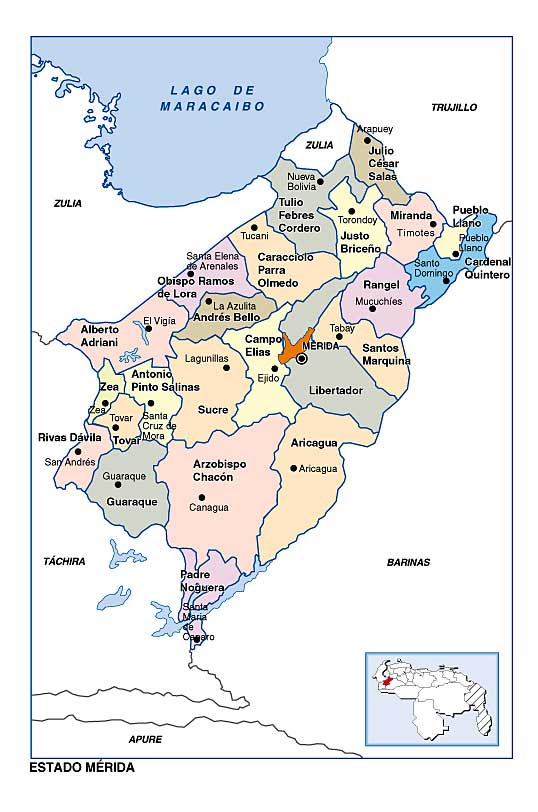
\includegraphics[scale=0.5]{merida.jpg}
	 \caption{Mapa del Estado M\'erida con sus municipios. Alcaldia del Estado M\'erida (2016)}
	 \end{figure}

\subsection{Lenguaje R para el computo estad\'istico}

El entorno de programaci\'on R es un clon de los lenguajes S y S-plus, de tal forma que muchos programas escritos en S y S-plus pueden ejecutarse en R sin modificaciones. S y S-plus son lenguajes de muy alto nivel diseñados para: La exploraci\'on y visualizaci\'on de datos; el modelado estad\'istico; y la programaci\'on con datos. \\

R es un entorno de programaci\'on para el an\'alisis estad\'istico y gr\'afico de datos, que cada vez se hace m\'as popular entre los investigadores de todas las disciplinas. Tiene muchas ventajas y es oportuno y pertinente para los investigadores de cualquier \'area del saber. \\

Como software libre es aprobado por varios motivos: trasmite valores socialmente positivos (libertad individual, conocimiento compartido, solidaridad y cooperaci\'on); se aproxima al m\'etodo cient\'ifico, porque permite el examen y mejora del c\'odigo desarrollado por otros ususarios y la reproducibilidad de los resultados obtenidos; pueden adquirirse de manera legal y gratuita copias del programa, sin necesidad de licencias personales o acad\'emicas. \\

Aparte de su faceta de software libre, R tiene algunas ventajas espec\'ificas: por ejemplo, su sintaxis b\'asica es sencilla e intuitiva, lo que se traduce en un aprendizaje r\'apido y c\'omodo; adem\'as, tiene una enorme comunidad de usuarios, estructurada alrededor de la \textit{Comprensive R Archive Network}, CRAN,lo que desarrolla cada d\'ia nuevos paquetes que extienden sus funcionalidades y cubren casi todas las necesidades computacionales y estad\'isticas de un cient\'ifico.

\subsection{Adquisici\'on y licencia}

El entorno R es un software libre en c\'odigo fuente bajo la definici\'on dada en la licencia GNU (General PublicLicense) de la FSF (Free software fundation), el cual puede ser descargado ya sea como c\'odigo fuente o como un ejecutable para los sistemas operativos Linux, Windows o MacOS.

\subsection{Interfaz de usuario}

La interacci\'on con el usuario se basa en una interfaz de usuario llamada RStudio, ambiente de desarrollo integrado que permite una interacci\'on r\'apida y amigable con R, adem\'as del desarrollo de c\'odigo de forma interactiva.

\begin{figure}[H]
\centering
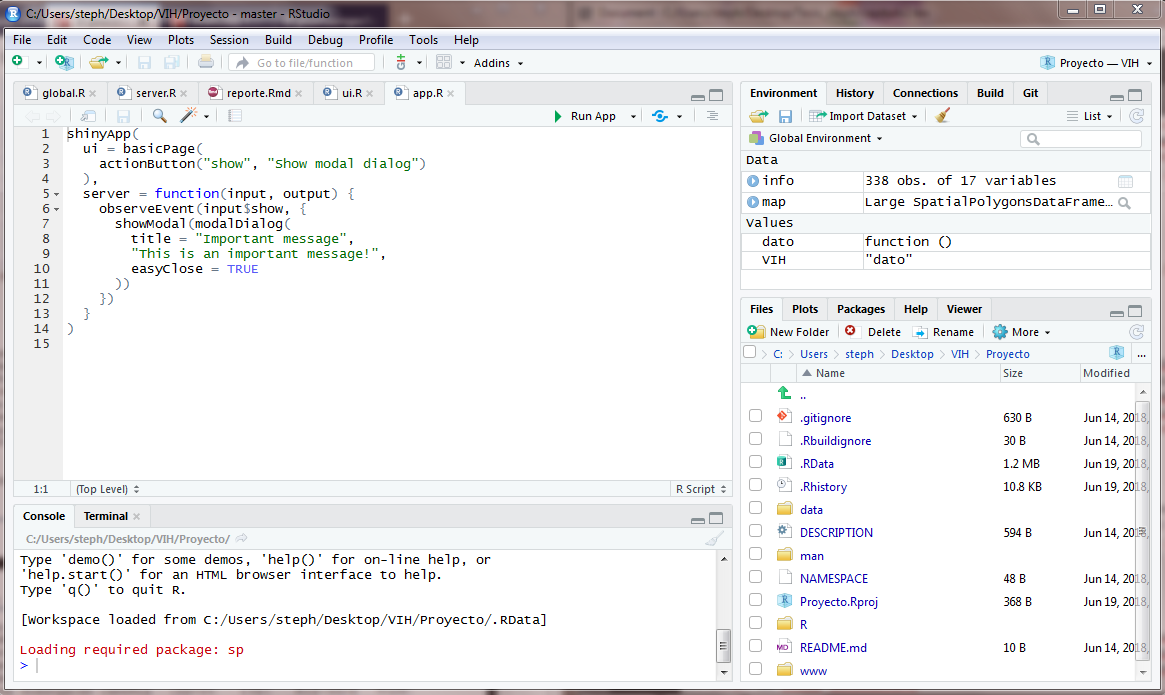
\includegraphics[scale=0.4]{RStudio.PNG}
\caption{Interfaz de RStudio (Versi\'on 1.1.453)}
\end{figure}

\subsection{Lenguaje de programaci\'on}

En su gram\'atica, la sintaxis del lenguaje R es similar a la de C y C++, pero su sem\'antica sigue los paradigmas de la programaci\'on funcional y la programaci\'on orientada a objetos, lo que implica que el lenguaje tiene la capacidad de manipular directamente los objectos del lenguaje, aplicar reglas de sustituci\'on y evaluar expresiones. \citet{grun}

R es un lenguaje orientado a objetos, tal que, inclusive los tipos m\'as b\'asicos de datos, tales como: booleanos, enteros, reales, caracteres, vectores, matrices, listas y hojas de datos son objetos mismos. Esta caracter\'istica permite que el usuario interact\'ue de forma transparente, ya que las llamadas se realizan a funciones gen\'ericas, como print, summary o plot, las cuales determinan internamente que m\'etodo debe ser llamado dependiendo de la clase de objetos a las que pertenecen sus argumentos. \\

R soporta internamente dos implementaciones para la programaci\'on orientada a objetos llamadas S3, que fue diseñado para uso interactivo, y S4, el cual supera las deficiencias de S3, y adiciona nuevos elementos. Adicionalmente, el usuario puede definir sus propias clases y los m\'etodos asociados a ellas.\\

\subsection{Shiny}

Shiny es un paquete R que facilita la creaci\'on de aplicaciones web interactivas (aplicaciones) directamente desde R. Las aplicaciones Shiny est\'an contenidas en un solo script llamado app.R. La secuencia de comandos app.R ubicado en un directorio (por ejemplo, nuevo/) y la aplicaci\'on se puede ejecutar con runApp ("nuevo").\\

app.R tiene tres componentes:

   \begin{itemize}
     \item un objeto de interfaz de usuario
     \item una funci\'on de servidor
     \item una llamada a la funci\'on shinyApp
     \end{itemize}

El objeto de la interfaz de usuario (ui) controla el diseño y la apariencia de la aplicaci\'on. La funci\'on del servidor contiene las instrucciones que la computadora necesita para construir la aplicaci\'on. Finalmente, la funci\'on shinyApp crea objetos de la aplicación Shiny desde un par de UI / servidor expl\'icito.

\begin{figure}[H]
\centering
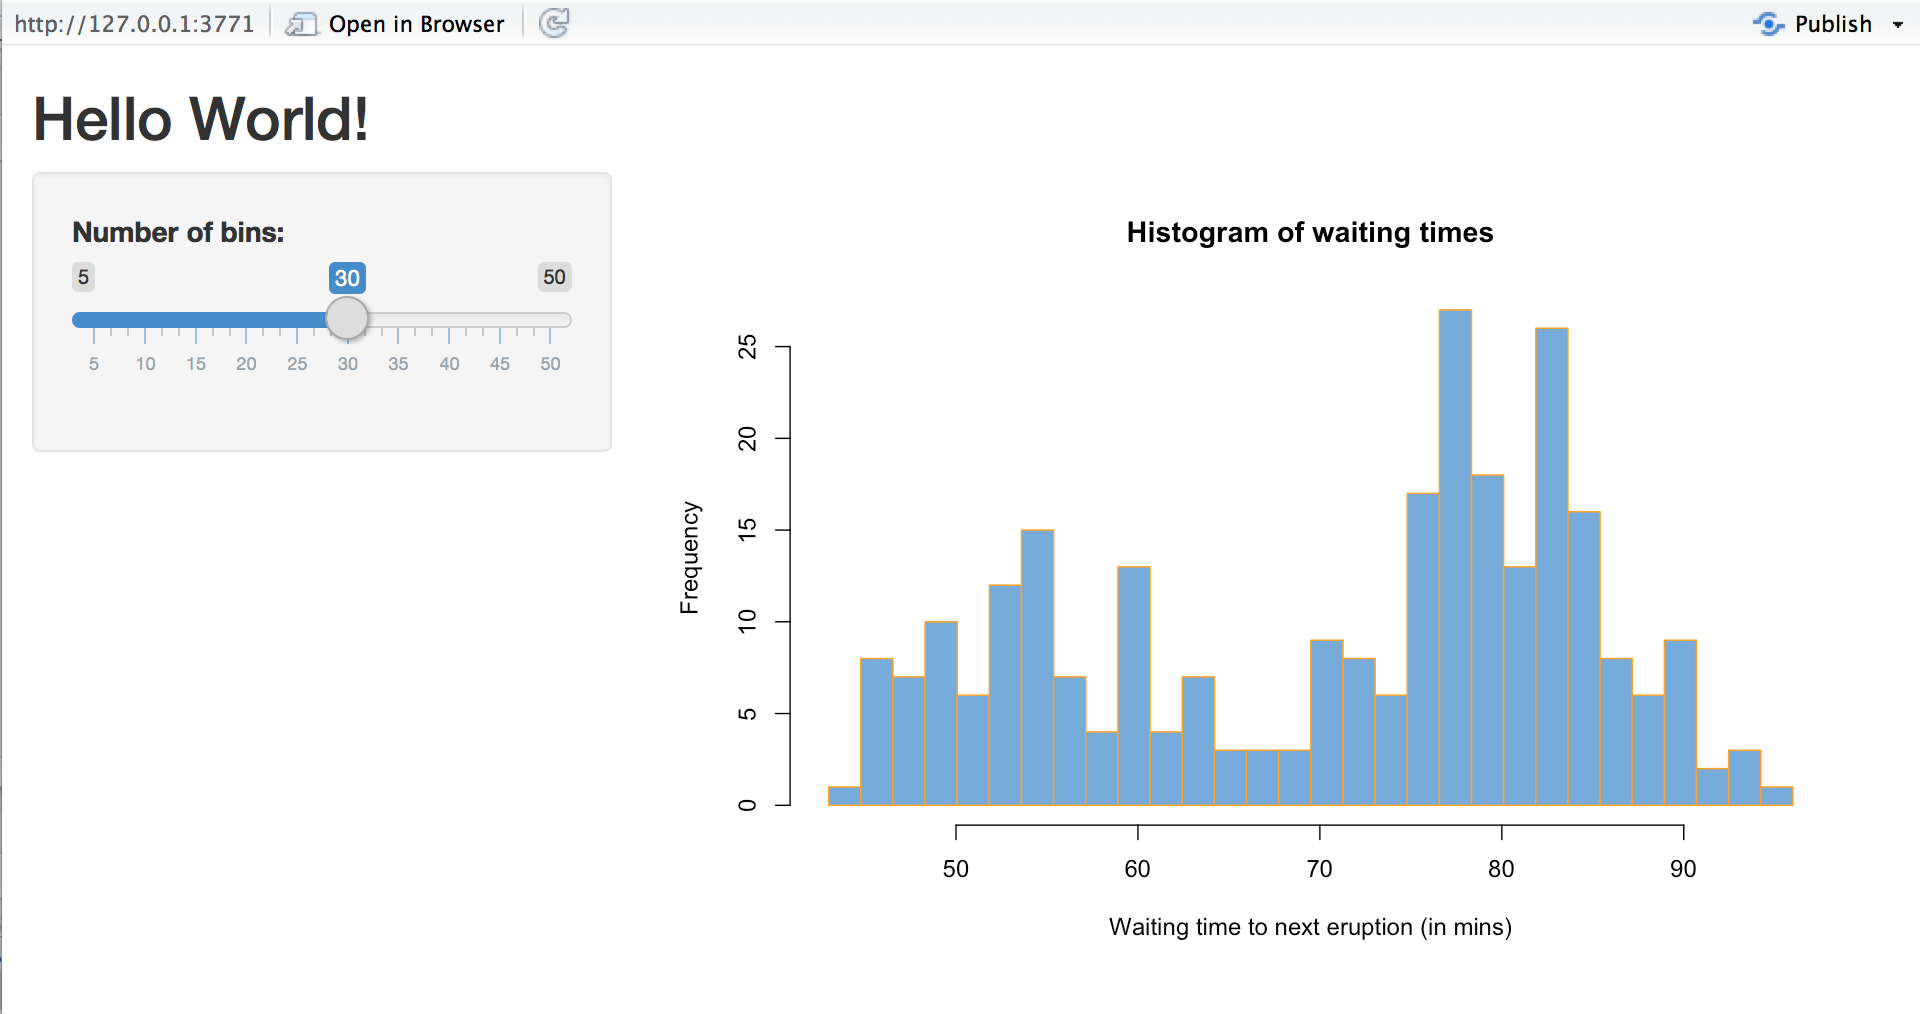
\includegraphics[scale=0.5]{shiny.png}
\caption{Aplicaci\'on en Shiny}
\end{figure}
